
\begin{figure}[h!]

  
    \begin{center}
    %\includegraphics[width=0.9\linewidth]{2020_www_graph_qa/figures/model_architecture-052119-evening.pdf}
    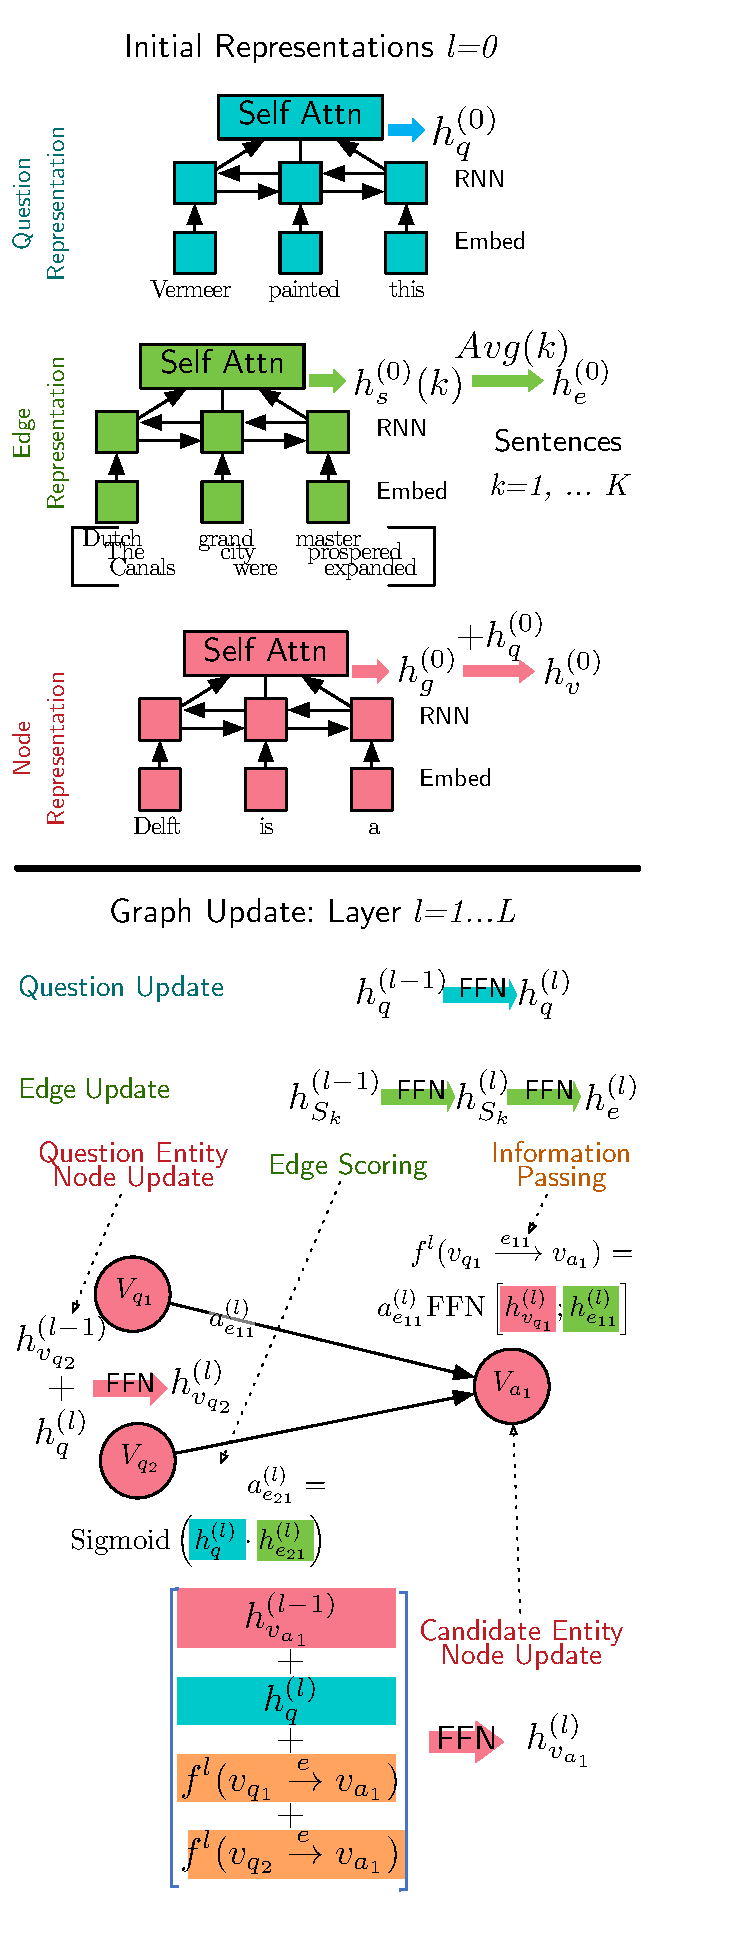
\includegraphics[width=0.86\linewidth]{2020_www_delft/figures/model}
    \end{center}
    \caption{Model architecture of \name{}'s \abr{gnn}. The left side
      shows the initial representation of the network. The right side
      illustrates the graph update.  }
    \label{fig:model}
\end{figure}

\section{Free-text Graph Modeling}
\label{sec:model}
%and what is its targeted output. Connect your discuss with last section}


Given the question $\mathcal{X}_q$ and the grounded free-text graph
$G$ from Section~\ref{sec:evidence}, the goal is to find the correct
answer node from the \rightnode{}s.  Recently several \abr{gnn} based
approaches~\cite{tu-etal-2019-multi, de2018question} answer questions
by modeling the knowledge graph.
%
%However, our free-text knowledge graph is unlike traditional knowledge graphs: (1) The nodes include textual 
%features of both question and node gloss; (2) Other than previous weighted or typed edges than can be represented as either adjacent matrix 
%or fixed embedding, an \name{}'s graph edge includes multiple free-text sentences. 
Unlike previous approaches that represent graph nodes and edges as fixed embeddings, 
\name{} adopts a \abr{gnn} to find the answer using  
a free-text knowledge graph.
We make the following motivating observations:
%that motivate us to design a
%specific \abr{gnn} model:


\paragraph{Graph Connectivity}

The correct \rightnode{} usually has many connections to \leftnode{}s.
%
For example, in Figure~\ref{fig:graph}, the correct \rightnode{}
\candidate{Delft} connects to all three question \leftnode{}s.
%
Thus, a correct \rightnode{} should \textit{aggregate} information
from multiple \leftnode{}s.


\paragraph{Edge Relevance}
The \tweennode{}s with sentences ``closer'' to the question
are likely to be more helpful to answering.
%
For example, in Figure~\ref{fig:graph}, the \leftnode{}
\question{The Little Street} has two edges to \rightnode{}s
\candidate{Delft} and \candidate{Amsterdam}, but the \tweennode{} with sentence
``\question{The Little Street} is one of only three paintings of views of \candidate{Delft}''
is more similar to the question.
The model needs to prioritize \tweennode{}s that are similar to the question.

\paragraph{Node Relevance}

In addition to relevant edges, we also use node
information to focus attention on the right \rightnode{}.
%
One aspect is ensuring we get the entity type correct (e.g., not
answering a place like \candidate{Uluru} to a ``who'' question like
``who took managing control of the Burra Burra mine in 1850?'').
%
For both \leftnode{} and \rightnode{}, we use entity gloss sentences
as node features.
%
For example, the gloss of the candidate entity node says
``\candidate{Delft} is a Dutch city'', which aligns what the question
asks (``this dutch city'').
%
Similarly, a \leftnode{} whose gloss sentence better matches a
question are more likely to contain the clues for the answer.

\paragraph{Iterative Refinement}

Figure~\ref{fig:model} illustrates the architecture of \name{}'s
\abr{gnn}.
%
A key component of the \abr{gnn} is that multiple layers ($^{(l)}$)
refine the representations of \rightnode{}s, hopefully focusing on the
correct answer.

The first layer learns the initial representation of the nodes and
edges, using their textual features and the relevance to the question
(Section~\ref{sec:init}).
%
Each successive layer combines this information, focusing on the
\tweennode{}s and \rightnode{}s that can best answer the question
(Section~\ref{sec:prop}).
%
The final layer scores the \rightnode{}s to produces an answer
(Section~\ref{sec:ans}).

\subsection{Initial Representations}
\label{sec:init}

We start with representations for questions, \leftnode{}s,
\rightnode{}s, and \tweennode{}s (\abr{gnn} layer~0).  These
representations are combined in subsequent layers.

\paragraph{Question and Node Representation}

Each question $\mathcal{X}_q$ and node gloss (both \rightnode{} and \leftnode{}) $\mathcal{X}_{g}$ 
is a sequence of word tokens $\mathcal{X} = (x_1,\dots, x_n)$.  Individual word embeddings $(\mathbf{E}_{x_1},\dots,
\mathbf{E}_{x_n})$ become a sequence representation~$\mathbf{h}_q^{(0)}$ ($\mathbf{h}_g^{(0)}$) using a 
Recurrent neural network (\abr{rnn}) with a self-attention (\abr{self-attn}) layer:
\begin{equation}
\mathbf{h}_{x_u} = \rnn{\mathbf{E}_{x_1},\dots, \mathbf{E}_{x_n}}
\end{equation}
where $u$ is token position of sequence~$\mathcal{X}$.  A
self-attention layer over the \abr{rnn} hidden layer first weights the hidden states
by a learnable weight vector $\mathbf{w}_x$
\begin{equation}
  a_{x_u} = \softmax{\mathbf{w}_x \cdot \mathbf{h}_{x_u}},
\label{eq:self_attn}
\end{equation}
then a final representation ${h}_x^{(0)}$ is a weighted average of 
all hidden states
\begin{equation}
\mathbf{h}_x^{(0)} = \sum_u a_{x_u}  \mathbf{h}_{x_u} .
\end{equation}

The node representation $\mathbf{h}_{v}^{(0)}$ of each node~$v~\in V$
is a sum of gloss representation $\mathbf{h}^{(0)}_{g}$ 
and question representation $\mathbf{h}_q^{(0)}$.
\begin{equation}
    \mathbf{h}_{v}^{(0)} = \mathbf{h}^{(0)}_{g} + \mathbf{h}_q^{(0)}.
\end{equation}
The representation $\mathbf{h}_{v}^{(0)}$ is applied to both question
entity nodes $\mathbf{h}_{v_q}^{(0)}$ and candidate answer nodes
$\mathbf{h}_{v_a}^{(0)}$.





\paragraph{Edge Representation}

Effective \tweennode{}s in \name{} should point from entities
mentioned in the question to the correct \rightnode{}.
%
We get the representation $\mathbf{h}_{e}^{(0)}$ of edge $e~\in E$
by first embedding each edge sentence $S(k)$'s tokens $\mathcal{X}_{s} = (s_1, ..., s_n)$
%The representation $\mathbf{h}_{e_{ij}}^{(0)}$ of edge $e_{ij}$
%
%The initial representation $\mathbf{h}_{e_{ij}}^{(0)}$ of edge $e_{ij}$ starts with
%the embedding of each evidence sentences' tokens $\mathcal{S}_{ij}({k}) = (s_1, ..., s_n)$ 
into $(\mathbf{E}_{s_1}, ..., \mathbf{E}_{s_n})$, then encoding with a \abr{rnn} layer:
\begin{align}
\mathbf{h}_{s_u} &= \rnn{\mathbf{E}_{s_1}, ..., \mathbf{E}_{s_n}}.
\end{align}
%To reflect the importance of each token position $u$ to the question, 
Then we fuse the question information into each edge sentence.
An inter attention layer~\cite{seo2016bidirectional} based on the question representation
$\mathbf{h}_q^{(0)}$ first weights each sentence token position $u$
\begin{equation}
  a_{s_u} = \softmax{\mathbf{h}_{s_u} \cdot \mathbf{h}_q^{(0)}};
\end{equation}
the weight is then combined into the question-aware edge sentence $k$'s representation $\mathbf{h}_{s}(k)$:
\begin{equation}
\mathbf{h}_{s}^{(0)}(k) = \sum_u a_{s_u} \mathbf{h}_{s_u}.
\end{equation}
Now that the edges have focused on the evidence that is useful to the question, we
average all edge sentences'
representations $\mathbf{h}_{s}^{k}$ 
into a single edge representation
\begin{align}
    \mathbf{h}_{e}^{(0)} &= \avg{\mathbf{h}_{s}^{(0)}(k)}{k}.
\end{align}

\subsection{Graph Update}
\label{sec:prop}


Given the initial representation of the question~$\mathbf{h}_q^{(0)}$,
nodes~$\mathbf{h}_{v}^{(0)}$, and edges~$\mathbf{h}_{e}^{(0)}$,
\name{}'s \abr{gnn} updates the representations through stacking
multiple layers.  It passes the representations from the question
nodes to the candidate nodes by combining multiple evidence edges'
information.
%
After this, the representations of the candidate nodes
in the final layer accumulates information from the question nodes
($v_q$), the question text ($q$), the evidence edges ($e_{ij}$), and
previous candidate representations.
%
These updated node representations are then used to calculate the answer scores.
% Once the propagation is complete, the
% final layer's representations of candidates nodes are used for answer ranking.

For each layer $l$, \name{}'s \abr{gnn} first updates the question and
edge representation with a feed forward network (\abr{ffn}) layer
(\textit{Representation Forwarding}), then it scores each edge by its
relevance to the question (\textit{Edge Scoring}), finally passing the
information (\textit{information passing}) from the question entity
nodes (\textit{Question Entity Nodes Update}) to candidate entity
nodes (\textit{Answer Entity Nodes Update}).
%
We discuss updates going from top to bottom in Figure~\ref{fig:model}.

\paragraph{Question Entity Nodes Update}

\leftnode{}s' representations $\mathbf{h}_{v_q}^{(l)}$ combine the question representation~$\mathbf{h}_q^{(l)}$ and the previous layer's
node representation~$\mathbf{h}_{v_q}^{(l-1)}$, 
\begin{align}
\mathbf{h}_{v_q}^{(l)} &= \ffn{\mathbf{h}_{v_q}^{(l-1)} + \mathbf{h}_q^{(l)}}.
\end{align}


\paragraph{Questions and Edges}

The representations of questions ($q$) and edges ($e$)---initially
represented through their constituent text in their initial
representation---are updated between layer $l-1$ and $l$ through a
feedforward network.
%
A question's single vector is straightforward,
\begin{align}
  \mathbf{h}_q^{(l)} = & \ffn{\mathbf{h}_q^{(l-1)}},
\end{align}
but edges are slightly more complicated because there may be multiple
sentences linking two entities together.
%
Thus, each individual sentence $k$ has its representation updated for layer~$l$,
\begin{align}
  \mathbf{h}_s^{(l)}{(k)}= & \ffn{\mathbf{h}_s^{(l-1)}{(k)}},
\end{align}
and those representations are averaged to update the overall edge representation,
\begin{align}
    \mathbf{h}_e^{(l)} = & \avg{\mathbf{h}_s^{(l)}{(k)}}{k}.
\end{align}



\paragraph{Edge Scoring}

Each edge has an edge score~$a_e$; higher edge scores indicate the
edge is more useful to answering the question.
%
The \abr{gnn} computes an edge score $a_e$ for each edge
representation $\mathbf{h}_e^{(l)}$ based on its similarity to this
layer's question representation:
%\jbgcomment{What does this do that attention does not?}
%\czcomment{There's no big differnce, at that time the GNN framework i use didn't support attn over outgoing edges.}
%scores each edge based on the relevance to the question:
\begin{align}
    a^{(l)}_e = & \text{Sigmoid}\left(\mathbf{h}_q^{(l)} \cdot \mathbf{h}_e^{(l)}\right).
\label{eq:edge-score}
\end{align}
%Where the Sigmoid is the activation function. \jbgcomment{This is a tautology.  Either cite, cut, or actually define Sigmoid function}
%The more relevance an edge is, the high importance it gets (Edge Relevance).

\paragraph{Information Passing}

The representation of the edge is not directly used to score
\rightnode{}s.
%
Instead, a representation is created from both the
source \leftnode{}~$\mathbf{h}_{v_q}^{(l)}$ and the combined
edges~$\mathbf{h}_e^{(l)}$ concatenated togther, feeds that through a
feed-forward network (to make the dimension consistent with previous layer and question representation), and weights by the edge score ($a_e$,
Equation~\ref{eq:edge-score}),
\begin{align}
f^{(l)}\left(v_q\xrightarrow{e} v_a\right)&= a_e^{(l)} \ffn{\left[\mathbf{h}_{v_q}^{(l)};\mathbf{h}_e^{(l)}\right]}.
\end{align}


\paragraph{Candidate Entity Nodes Update}

The updated representation for each \rightnode{} 
combines the previous layer's \rightnode{} representation, the question
representation, and the passed information. 
\begin{equation}
  \mathbf{h}_{v_a}^{(l)}= \text{\abr{ffn}}
   \left( \vphantom{\mathbf{h}_{v_a}^{(l-1)}} \right.
  \explain{previous}{\mathbf{h}_{v_a}^{(l-1)}}
                           + \explain{question}{\mathbf{h}_q^{(l)}} +
                           \explain{Information Passing}{\sum_{v_q \in V_q} f^{(l)}(v_q\xrightarrow{e} v_a)}
                              \left. \vphantom{\mathbf{h}_{v_a}^{(l-1)}} \right).
                         \end{equation}
After iterating through several \abr{gnn} layers, the candidate node
representations aggregate information from the question nodes, edges,
and candidate nodes themselves.

\subsection{Answer Scoring}
\label{sec:ans}

%After several layers' graph propagation, 
Finally, \name{} uses a multi-layer perception (\abr{mlp}) to score the \rightnode{} using the
final layer $L$'s representations,
\begin{equation}
p({v_a; G}) = \mbox{\sigmoid{}}\left(\mbox{\abr{mlp}}(\mathbf{h}^{(L)}_{v_a})\right).
\label{eq:node-update}
\end{equation}
The \abr{gnn} is trained using binary cross entropy
loss over all \rightnode{}s $v_a$.  At test time, it
chooses the answer with the highest $p({v_a, G})$.